\documentclass[journal,twoside,web]{ieeecolor}
\usepackage{jsen}
\usepackage{cite}
\usepackage{amsmath,amssymb,amsfonts}
\usepackage{graphicx}
\graphicspath{{../../results/figures/}{figures/}{./}}
\usepackage{textcomp}
\usepackage{wrapfig}
\usepackage{booktabs}
\usepackage{multirow}
\usepackage{url}
\usepackage{bm}
\usepackage{mathtools}
\usepackage{hyperref}
% ieeecolor already defines \proof, so amsthm is not loaded; LaTeX's own \newtheorem suffices.
\newtheorem{lemma}{Lemma}
\newtheorem{theorem}{Theorem}
\newtheorem{corollary}{Corollary}
% Public code + data repository (single source of truth)
\newcommand{\repourl}{https://github.com/Praveg432/OmniST}
\newcommand{\Risk}{r}
\markboth{\journalname, VOL. XX, NO. XX, XXXX 2026}
{Vashishtha: OmniST: Topology-Invariant Forecasting for Dynamic Sensor Networks}
\definecolor{abstractbg}{rgb}{0.89804,0.94510,0.83137}
\setlength{\fboxrule}{0pt}
\setlength{\fboxsep}{0pt}
\begin{document}
\title{OmniST: Topology-Invariant Forecasting for Dynamic Sensor Networks With Conformal Intervals at
Unseen Sensors}
\author{Praveg Vashishtha
\thanks{Manuscript submitted XX, 2026. This research did not receive any specific grant from funding agencies in the public, commercial, or not-for-profit sectors.}
\thanks{P. Vashishtha is with the Department of Computer Science and Engineering, Indian Institute
of Technology Patna, Patna 801106, India, and with Sopra Banking Software India, where he is a Senior
Software Development Engineer (e-mail: praveg\_pa2503mth259@iitp.ac.in).}}
\IEEEtitleabstractindextext{%
\fcolorbox{abstractbg}{abstractbg}{%
\begin{minipage}{\textwidth}%
\begin{wrapfigure}[12]{r}{3in}%
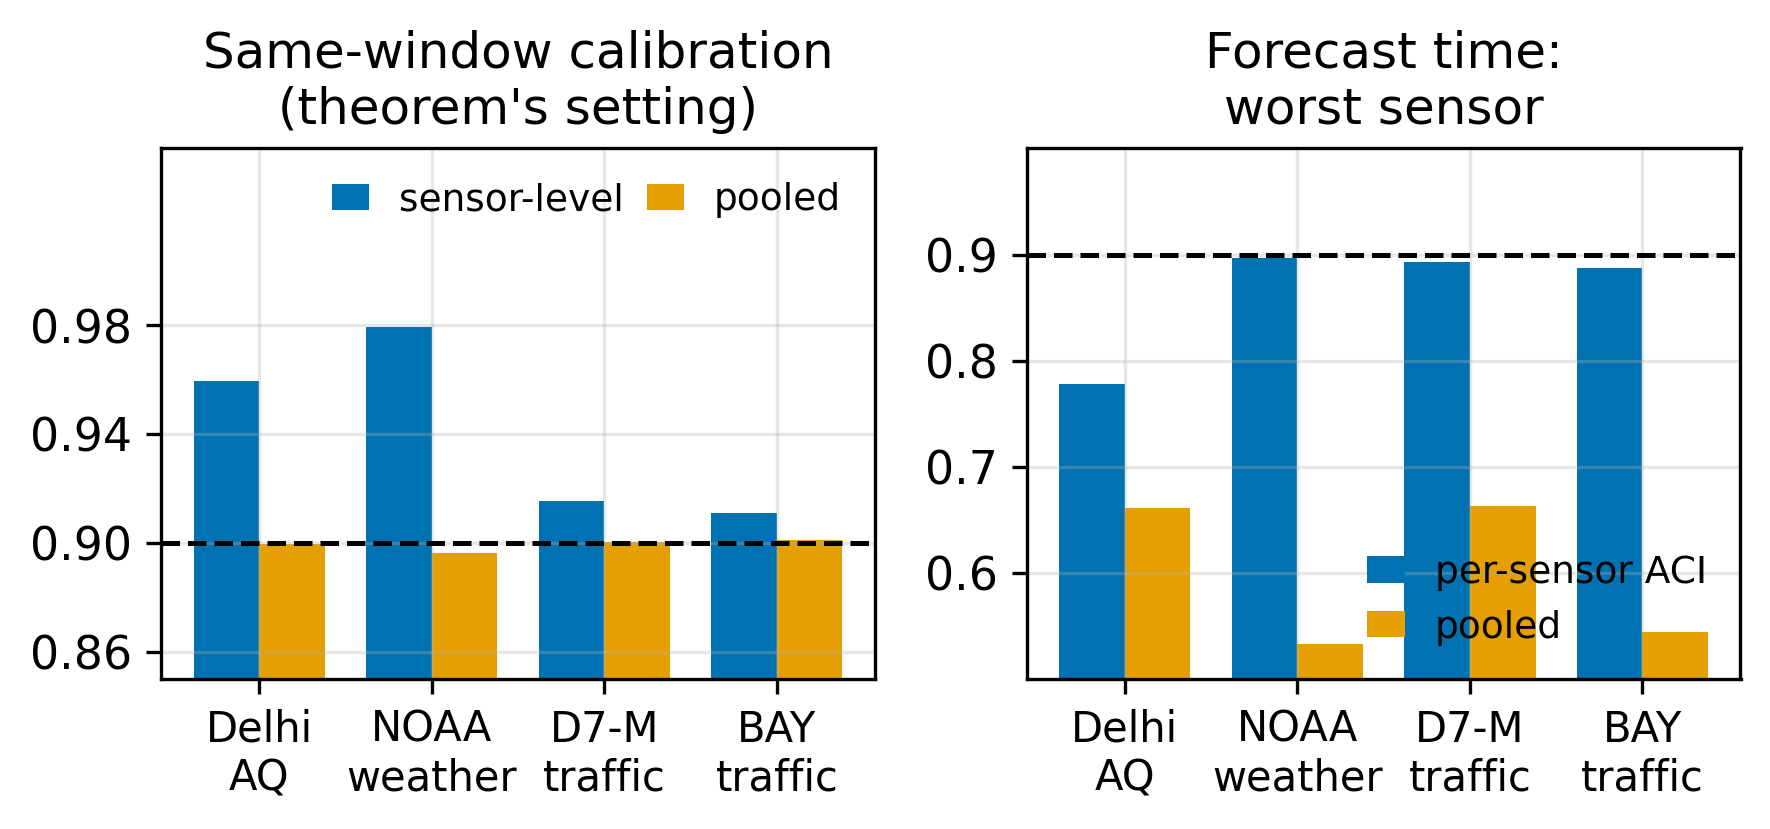
\includegraphics[width=3in]{graphical_abstract_jsen.png}%
\end{wrapfigure}%
\begin{abstract}
@@ABSTRACT@@
\end{abstract}
\begin{IEEEkeywords}
Conformal prediction, inductive prediction, sensor failure, sensor networks, spatiotemporal forecasting, uncertainty quantification.
\end{IEEEkeywords}
\end{minipage}}}
\maketitle
\section{Introduction}
\label{sec:introduction}
\IEEEPARstart{A}{n} operational sensor network rarely keeps the layout it was trained on. India's
Central Pollution Control Board adds air-quality stations every year~\cite{panja2026estgcn}, traffic
detectors fail, and weather stations go offline for maintenance. A forecaster serving such a network
has to keep working when a sensor disappears, and it has to produce a usable forecast, with an
honest statement of its uncertainty, at a sensor that was installed after the model was trained.

Spatiotemporal graph convolutional networks (STGCNs)~\cite{yu2018stgcn} forecast accurately on a
fixed network, but they encode it as a pre-computed $N\times N$ adjacency matrix. A sensor added after
training has no row or column in that matrix, so the model produces no forecast there, and removing a
trained sensor breaks the matrix product. Some implementations recompute the adjacency and can adapt,
but that is an engineering choice rather than something the formulation provides.

A point forecast at a new sensor is not enough for an operator, who also needs to know how far to
trust it. Split conformal prediction~\cite{vovk2005algorithmic,angelopoulos2023conformal} supplies
distribution-free intervals, but its guarantee depends on the calibration errors being exchangeable
with the error at the point being predicted. For a forecaster at a new sensor this is easy to get
wrong in two ways. If the calibration errors come from the sensors the model was trained on, they are
systematically different from the errors at a sensor it has never seen. And even with disjoint
calibration sensors, the thousands of errors one sensor produces over time are strongly dependent,
so the number of calibration \emph{points} overstates the information the calibration set carries.
The unit that can be exchangeable across a random choice of new sensor is the sensor.

This paper makes a design and an evidence contribution built around that observation.
\begin{enumerate}
\item \textbf{A forecaster with no dependence on the sensor count}
(Section~\ref{sec:architecture}): ``topology invariant'' in the sense that the model produces outputs for any
set of sensors.
\item \textbf{Two coverage guarantees with complementary scope, for intervals at new sensors.} A locality lemma
(Lemma~\ref{lem:locality}) makes a new sensor's error a function of its own data and its nearest
training-network neighbors. Theorem~\ref{thm:coverage} then gives finite-sample expected coverage at a randomly
drawn new sensor, with a correction counted in calibration \emph{sensors}; it needs random assignment and errors
from the evaluated window. Theorem~\ref{thm:aci} gives what the first cannot: coverage at forecast time for every
individual sensor, including named, distant and non-randomly chosen ones, in the long run and over any block of
windows. Exact single-window or location-conditional coverage is impossible without assumptions
(Section~\ref{sec:online-conformal}). Neither argument is new (hierarchical conformal
prediction~\cite{lee2023hcp}, conformal risk control~\cite{crc2024}, adaptive conformal
inference~\cite{gibbs2021aci}); the lemma makes them apply to a forecaster on a changing network, and the lemma
alone does not imply coverage, as the previous version of this work assumed.
\item \textbf{Measured scope and price of each guarantee on five real networks}, from models trained on disjoint
sensors: where each holds, where it is vacuous, its width cost, and the worst individual sensor
(Section~\ref{sec:results}). The usual pooled recipe averages near target but leaves the worst sensor at 0.53 to
0.81 at forecast time; per-sensor ACI raises it to about 0.89 on the traffic networks at no larger median width. On 70 weather
stations that were installed after training, every station was covered at least 0.88 (Section~\ref{sec:late}).
\item \textbf{What the architecture contributes}, against like-for-like forecasting baselines, seasonal-naive
forecasting and a coordinate-free shared per-sensor model.
\end{enumerate}
%% ====================================================================
\section{Method}
\label{sec:architecture}

\subsection{An Architecture With No Global Sensor Count}

OmniST satisfies one invariant: for any sensor $i$ the output $f(i)$ depends only on sensor $i$'s own
data and a fixed-size neighborhood $\mathcal{N}_k(i)$, never on the full set of sensors present.

\textbf{Coordinate tokens.} Each observation becomes a token
\begin{equation}
\mathbf{z}_i(t) = f_{\text{MLP}}(\phi_i, \lambda_i) + f_{\text{time}}(t) + W_f \mathbf{x}_i(t),
\end{equation}
where $f_{\text{MLP}}:\mathbb{R}^2\to\mathbb{R}^d$ is a 3-layer MLP on centered latitude and longitude,
$f_{\text{time}}$ encodes calendar features with sinusoidal harmonics, and $W_f$ projects the raw
measurements. No other sensor enters $\mathbf{z}_i(t)$. The centering constants of
$f_{\text{MLP}}$ were fixed for Delhi; for the other regions the coordinate input lies far outside the
intended range, so the learned coordinate embedding is better read as a sensor-identity feature than
as a geographic one. Section~\ref{sec:ablation} measures how much it matters.

\textbf{Neighbor attention.} Spatial context comes from the $k$ geographically nearest sensors,
\begin{equation}
\mathbf{z}_i' = \text{LayerNorm}\Big(\mathbf{z}_i + \sum_{j \in \mathcal{N}_k(i)} \alpha_{ij} W_v \mathbf{z}_j\Big),
\end{equation}
with $\mathcal{N}_k(i)$ found by Haversine distance at every forward pass and $\alpha_{ij}$ the
multi-head attention weights with a learned distance bias. We use a single attention layer, so the
receptive field of a sensor is exactly $\mathcal{N}_k(i)$. In the \emph{reference-restricted} mode
used for every coverage experiment, $\mathcal{N}_k(i)$ is searched only among the sensors of the
training network, so sensors outside it never influence one another.

\textbf{Per-sensor temporal model and head.} A bidirectional GRU processes each sensor's sequence
independently, and a 2-layer MLP maps the final state to the forecast horizon. The model has
${\sim}315$K parameters at $d{=}128$ and is trained with AdamW, cosine annealing, early stopping on
training-network validation windows, and the Peaks-Over-Threshold loss of~\cite{panja2026estgcn}.

\textbf{What a new sensor needs.} The input to the model at a sensor is that sensor's own recent
history. OmniST therefore forecasts at a sensor that has no \emph{training} history but has at
least one input window of observations. It does not address a location with no data at all.

\subsection{Setting for Coverage at New Sensors}
\label{sec:setting}

Let $\mathcal{T}$ be the training network and $\hat f$ the model fitted on data from $\mathcal{T}$
alone, including early stopping and any hyperparameter choice. Let $\mathcal{R}$ be a set of further
sensors that were not used in any way during fitting, observed over an evaluation window shared by
all of them. For $i\in\mathcal{R}$ let $\hat y_{i,u}$ be the forecast at the $u$-th of $U$
(window, horizon-step) points, computed by $\hat f$ from sensor $i$'s own input history and the
histories of its $k$ nearest sensors in $\mathcal{T}$. The nonconformity score is
$s_{i,u}=|\hat y_{i,u}-y_{i,u}|$ and the interval is $[\hat y_{i,u}-q,\ \hat y_{i,u}+q]$ (clipped at
zero for non-negative quantities, which cannot change coverage). The miscoverage at sensor $i$ is
\begin{equation}
\Risk_i(q)=\frac{1}{U}\sum_{u=1}^{U}\mathbf{1}\{s_{i,u}>q\},
\end{equation}
a non-increasing, right-continuous function of $q$ with values in $[0,1]$.

\subsection{Locality and Sensor-Level Coverage}
\label{sec:theory}

\begin{lemma}[Locality]
\label{lem:locality}
Let $S\ni i$ be any set of additional sensors present alongside $\mathcal{T}$, and let neighbors be
searched in $\mathcal{T}$ only. The forecast $\hat y_i$ depends on $(\mathcal{T},S)$ only through the
coordinates and history of sensor $i$ and of the $k$ sensors of $\mathcal{N}_k(i;\mathcal{T})$.
Consequently $\hat y_i$ is unchanged if sensors of $S\setminus\{i\}$ are added or removed, or if
sensors of $\mathcal{T}$ outside $\mathcal{N}_k(i;\mathcal{T})$ are added or removed.
\end{lemma}
\begin{proof}
The token of a sensor is a function of its own coordinates, time features and measurements. With one
attention layer, the output at $i$ aggregates the values of exactly $\mathcal{N}_k(i;\mathcal{T})$
with weights computed from $i$'s query, those neighbors' keys and the distances to them, and there is
no normalization across sensors. The GRU and the head act on each sensor separately. Nothing uses the
number of sensors or a sensor index. Ties in distance are broken by a fixed rule. \end{proof}

The lemma says what a score is a function of. It does not say that scores at calibration sensors
and at a new sensor have the same distribution, and so by itself it gives no coverage statement:
a model typically fits the sensors it was trained on better than sensors it never saw. What it does
establish is the structure the theorem needs. Every sensor of $\mathcal{R}$ is scored by one and the
same function, and the score of a sensor does not depend on which other new sensors are present.
We check the lemma numerically in the released tests: scoring many new sensors in one pass equals
scoring each alone added to $\mathcal{T}$, to $10^{-5}$, for both the exact and the scalable
neighbor search.

\begin{theorem}[Sensor-level coverage]
\label{thm:coverage}
Fix $\mathcal{T}$ and $\hat f$, and let $\mathcal{R}$ contain at least $n+1$ sensors. Draw $J$
uniformly from $\mathcal{R}$ and, given $J$, a uniformly random $n$-subset $\mathcal{C}$ of
$\mathcal{R}\setminus\{J\}$. For $\alpha\in(0,1)$ let
\begin{equation}
\hat q(\mathcal{C})=\inf\Big\{q\ge 0:\ \frac{1}{n+1}\Big(1+\sum_{i\in\mathcal{C}}\Risk_i(q)\Big)\le\alpha\Big\},
\end{equation}
with $\inf\emptyset=\infty$. Then $\mathbb{E}\big[\Risk_J(\hat q(\mathcal{C}))\big]\le\alpha$, the
expectation being over the draw of $(J,\mathcal{C})$.
\end{theorem}
\begin{proof}
Let $A=\mathcal{C}\cup\{J\}$. It is a uniformly random $(n+1)$-subset of $\mathcal{R}$, and given $A$
the sensor $J$ is uniform on $A$. Fix $A$. For $j\in A$ let $\hat q_{-j}$ be the threshold computed from
$A\setminus\{j\}$, and let $\tilde q=\inf\{q:\frac{1}{n+1}\sum_{i\in A}\Risk_i(q)\le\alpha\}$. The set
is non-empty because every $\Risk_i$ is zero beyond the largest score, and each $\Risk_i$ is
right-continuous, so the infimum is attained. Since $\Risk_j\le 1$,
\[
\tfrac{1}{n+1}\textstyle\sum_{i\in A}\Risk_i(q)\ \le\ \tfrac{1}{n+1}\big(1+\sum_{i\in A\setminus\{j\}}\Risk_i(q)\big)\quad\text{for all }q,
\]
so every $q$ admissible for $\hat q_{-j}$ is admissible for $\tilde q$, and $\hat q_{-j}\ge\tilde q$.
As $\Risk_j$ is non-increasing, $\Risk_j(\hat q_{-j})\le\Risk_j(\tilde q)$. Averaging over $j\in A$,
\[
\mathbb{E}\big[\Risk_J(\hat q(\mathcal{C}))\mid A\big]=\tfrac{1}{n+1}\textstyle\sum_{j\in A}\Risk_j(\hat q_{-j})
\le\tfrac{1}{n+1}\sum_{j\in A}\Risk_j(\tilde q)\le\alpha .
\]
Taking the expectation over $A$ completes the proof. \end{proof}

The argument is the conformal risk control argument~\cite{crc2024} with the per-sensor miscoverage
$\Risk_i$ as the loss. Because every sensor contributes the same number $U$ of points, the average
$\frac1n\sum_{i\in\mathcal{C}}\Risk_i(q)$ is the fraction of all pooled calibration errors above $q$,
so the rule is a pooled quantile with a different correction.

\begin{corollary}[Pooled form and price]
\label{cor:pooled}
Let $\alpha_n=(\alpha(n+1)-1)/n$. Then $\hat q$ is the $\lceil(1-\alpha_n)\,nU\rceil$-th smallest of the
$nU$ pooled calibration errors, and is infinite exactly when $n<1/\alpha-1$.
\end{corollary}
The usual split-conformal correction instead uses $(nU+1)$, that is $\alpha_{nU}\approx\alpha$, which
treats the $nU$ errors as exchangeable. Here the correction is counted in sensors: at $\alpha=0.1$ at
least $9$ calibration sensors are needed for a finite interval, $19$ at $\alpha=0.05$, and $4$ at
$\alpha=0.2$. This is the price of a distribution-free statement when sensors, not points, are
the exchangeable units. With the same number of points per sensor, the rule is exactly the threshold of
hierarchical conformal prediction~\cite{lee2023hcp}.

\textbf{What the theorem does and does not say.}
\emph{(A1) Random assignment.} The probability is over which sensor plays the new one. It is a
statement about a sensor drawn at random from $\mathcal{R}$, not about a named sensor, and not
conditional on location.  A new sensor that is systematically different
from the calibration sensors, for instance far outside the network, is outside the theorem;
weighted conformal prediction~\cite{tibshirani2019covshift,barber2023nexcp} is the route there, and
Sections~\ref{sec:deployable} and \ref{sec:late} test far and late-installed sensors.
\emph{(A2) Common window.} Calibration and test errors come from the same evaluation window. This is
the setting in which the theorem holds, and it cannot be run at forecast time: when a forecast for
window $t$ is issued, the calibration sensors' errors for window $t$ are not yet known. With
calibration restricted to earlier windows the errors of different windows are not exchangeable and the
theorem says nothing; Theorem~\ref{thm:aci} (Section~\ref{sec:online-conformal}) covers that case per sensor.
\emph{(A3) Independence of the model.} $\hat f$ is fitted without $\mathcal{R}$.
\emph{(A4) Own history.} Every sensor has its input window.
The bound is on average coverage over the $U$ points of a sensor, not per time step and not per sensor.

\textbf{Topology change.} If a set $D\subset\mathcal{T}$ of reference sensors goes offline, by
Lemma~\ref{lem:locality} only the sensors of $\mathcal{R}$ with a neighbor in $D$ change their score.
Rescoring them against the reduced network and recalibrating gives Theorem~\ref{thm:coverage} for the reduced
network with the same $\hat f$; the earlier claim that no recalibration is needed holds only for the cached
scores of unaffected sensors.

\subsection{A Guarantee at Forecast Time, for Every Sensor}
\label{sec:online-conformal}
Theorem~\ref{thm:coverage} is silent about calibration that uses only errors observed before the
forecast. For the forecast of window $t$ we form the threshold from the calibration sensors' errors of
earlier windows only: \emph{static} (windows before a fixed start $t_0$), \emph{expanding} (all windows
before $t$), or \emph{rolling} (the previous $L$ windows), with the sensor-level or pooled correction.
None of these has a guarantee. A guarantee that needs neither exchangeability nor a random choice of
sensor comes from Adaptive Conformal Inference (ACI)~\cite{gibbs2021aci}, applied separately to each new
sensor $j$. Let $Q_t(a)$ be the rolling sensor-level threshold computed at working level $a$, with
$Q_t(a)=+\infty$ when $a(n+1)<1$ and the empty interval when $a\ge 1$. Set $\alpha_{t_0}=\alpha$,
issue $\hat y\pm Q_t(\alpha_t)$ for window $t$, and update
\begin{equation}
\alpha_{t+1}=\alpha_t+\gamma(\alpha-e_t),
\end{equation}
where $e_t\in[0,1]$ is the share of sensor $j$'s points of window $t$ outside its interval. Windows
advance by the horizon, so $e_t$ is known at the origin of window $t+1$.

\begin{theorem}[Per-sensor long-run coverage]
\label{thm:aci}
For every sensor $j$, every $T\ge1$ and every sequence of errors,
$\big|\frac1T\sum_{t=t_0}^{t_0+T-1}e_t-\alpha\big|\le\frac{\max(\alpha,1-\alpha)+\gamma}{\gamma T}$.
\end{theorem}
\begin{proof}
$Q_t$ is non-increasing in $a$, gives $e_t=0$ when $\alpha_t<1/(n+1)$ and $e_t=1$ when $\alpha_t\ge1$. Hence
$\alpha_t$ rises whenever it is below $1/(n+1)$ and falls whenever it is at least $1$, by at most $\gamma$ per
step, so $\alpha_t\in[-\gamma,1+\gamma]$. Summing the update,
$\alpha_{t_0+T}-\alpha=\gamma\sum_t(\alpha-e_t)$, and $|\alpha_{t_0+T}-\alpha|\le\max(\alpha,1-\alpha)+\gamma$.
\end{proof}

This is Gibbs and Cand\`es' argument~\cite{gibbs2021aci} with fractional errors, and we do not claim it.
What it gives here is the statement Theorem~\ref{thm:coverage} lacks: it holds at forecast time, for a
named sensor, for one far from the network, and under drift. Its price is that it is about the long-run
average over that sensor's own windows, with slack of order $1/(\gamma T)$, so it is informative only
after enough windows, and some windows receive an infinite interval while $\alpha_t$ is low. An earlier
draft of this work clipped $\alpha_t$ to $[0.005,0.995]$, which voids the bound; the results here use the
unclipped update. $L$, $t_0=L$ and $\gamma\in\{0.1,0.5\}$ were fixed before the results were seen.
\begin{corollary}[Blocks of windows]
\label{cor:block}
For every sensor $j$, every $k\ge1$ and every block of $k$ consecutive windows,
$\big|\frac1k\sum_{t=s}^{s+k-1}e_t-\alpha\big|\le\frac{1+2\gamma}{\gamma k}$.
\end{corollary}
\begin{proof}
Both $\alpha_s$ and $\alpha_{s+k}$ lie in $[-\gamma,1+\gamma]$, so $|\alpha_{s+k}-\alpha_s|\le1+2\gamma$, and
$\alpha_{s+k}-\alpha_s=\gamma\sum_{t=s}^{s+k-1}(\alpha-e_t)$. \end{proof}
\emph{Single windows and locations.} Coverage at one window, or conditional on the new sensor's location, cannot
be guaranteed exactly by any distribution-free method: a method valid conditionally on a point must, for
continuous data, return intervals of infinite expected length~\cite{vovk2012conditional,lei2014distribution,barber2021limits}.
We therefore guarantee what is attainable: coverage per sensor, and hence per location, over any block of $k$
windows, with certificate $1-\alpha-(1+2\gamma)/(\gamma k)$, which is informative only for long blocks.
Theorem~\ref{thm:coverage} applied within groups of sensors (for example by distance from the network) gives
group-conditional coverage when each group has at least $1/\alpha-1=9$ calibration sensors. Tracking local
shifts more tightly is the aim of strongly adaptive variants~\cite{gibbs2024dtaci}, which we do not implement.

@@RESULTS@@
